\documentclass[a4paper,12pt,french]{article}

\usepackage[cours]{../../../Style}

%\usepackage[theorems]{tcolorbox}

%\newtcbtheorem
%{defi}{Définition}
%{colback=red!5,colframe=red!60!black!80,fonttitle=
%\sffamily\bfseries}{th}

% Début du document
%%%%%%%%%%%%%%%%%%%
\begin{document}

\title{Suites arithmétiques et géométriques}
\maketitle

\begin{programme}
\item Suites arithmétiques: évolutions absolues constantes (croissance linéaire).
\item Suites géométriques: évolutions relatives constantes (croissance exponentielle).
\begin{itemize}
\item Relation de récurrence
\item Sens de variation
\item Représentation graphique
\end{itemize}
\item Compétences
\begin{itemize}
\item Reconnaitre si une situation relève d'un modèle discret de croissance linéaire ou exponentielle.
\item Conjecturer, à partir de sa représentation graphique, la nature arithmétique ou géométrique d'une suite.
\item Démontrer qu'une suite est arithmétique ou géométrique.
\item Déterminer le sens de variation d'une suite arithmétique ou géométrique à l'aide de la raison.
\end{itemize}
\end{programme}

\section{Suites arithmétiques}

\subsection{Généralités}

\begin{defin}
Un premier terme, un nombre r appelé raison et la relation $a_{n+1}=a_n+r$. 
\end{defin}

\begin{rmq}
On passe d'un terme au suivant en ajoutant toujours le même nombre. La différence entre deux termes successifs vaut toujours $r$: $a_{n+1}-a_n=r$.

\begin{center}
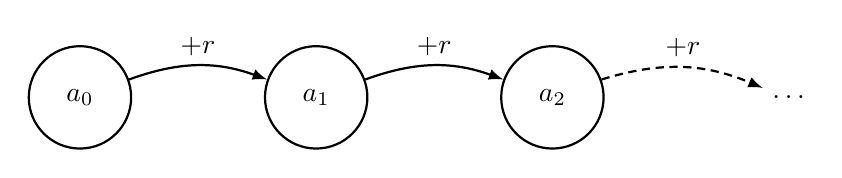
\begin{tikzpicture}[scale=1]
\node[draw,circle,thick, minimum size=13mm] (W0) at (-3,0) {$a_0$};
\node[draw,circle,thick, minimum size=13mm] (W1) at (0,0) {$a_1$};
\node[draw,circle,thick, minimum size=13mm] (W2) at (3,0) {$a_2$};
\node (W5) at (6,0) {$\ldots$};
\draw[->,>=latex,thick] (W0) to[bend left=20] node[midway,above]{$+r$} (W1);
\draw[->,>=latex,thick] (W1) to[bend left=20] node[midway,above]{$+r$} (W2);
\draw[->,>=latex,thick,densely dashed] (W2) to[bend left=20] node[midway,above]{$+r$} (W5);
\end{tikzpicture}
\end{center}

\end{rmq}

\begin{ex}
Soit $u$ la suite arithmétique de premier terme $u_0=5$ et de raison $r=-2$. Alors:
$$
\begin{aligned}
u_1&=u_0-2=3\\
u_2&=u_1-2=1\\
u_3&=u_2-2=-1\\
u_4&=\ \ldots
\end{aligned}
$$
\end{ex}

\begin{propr}
Lorsqu'on représente graphiquement une suite arithmétique, les points obtenus sont alignés.
\end{propr}

\begin{ex}
\begin{center}
\begin{tikzpicture}[scale=\echellepgf]
\begin{axis}[
styleglobal,
hauteurproptick,
width=0.9*\echellepgfinv*\linewidth,
xmin=0, xmax=10.5,
ymin=-2.5, ymax=3.5,
xtick distance=1,
ytick distance=1
]
\addplot[samples=11,ultra thick,domain=(0:10),only marks,mark options={stylepoint,color=blue}]{-0.5*x+3};
\end{axis}
\end{tikzpicture}
\end{center}

On a représenté une suite $u$ ci-dessus. Son premier terme $u_0$ vaut $3$ et pour passer d'un terme au suivant, on retire $0.5$: $r=-0.5$. La suite $u$ est donc une suite arithmétique de premier terme $3$ et de raison $-0.5$.
\end{ex}

\begin{methode}
Pour s'assurer qu'une suite \textbf{semble} arithmétique, on calcule la différence entre deux termes successifs, et l'on doit toujours trouver le même nombre (la raison).
\end{methode}

\begin{ex}
On se donne deux suites $u$ et $v$, dont quelques valeurs sont décrites dans le tableau ci-dessous:
\begin{center}
\begin{tabularx}{0.5\linewidth}{|c|*{4}{Y|}} \hline
$n$ & 0 & 1 & 2 & 3 \\ \hline
$u_n$ & 5 & 9 & 13 & 17 \\ \hline
$v_n$ & 3 & 12 & 20 & 29 \\ \hline
\end{tabularx}
\end{center}
\end{ex}

\subsection{Variations des suites arithmétiques}

\begin{prop}
\begin{itemize}
\item Si $r > 0$, alors la suite $a$ est croissante.
\item Si $r < 0$, alors la suite $a$ est décroissante.
\item Si $r = 0$, alors la suite $a$ est constante.
\end{itemize}
\end{prop}

\begin{ex}
Soit $a$ la suite arithmétique définie par $a_0=13$ et pour tout $n \in \N, a_{n+1}=a_n-5$. La raison de cette suite est $r=-5<0$ donc $a$ est décroissante.
\end{ex}

\section{Suites géométriques, cas positif}

\subsection{Généralités}

\begin{defin}
Un premier terme, un nombre $q$ appelé raison et la relation de récurrence $g_{n+1}=q \times g_n$.

\begin{center}
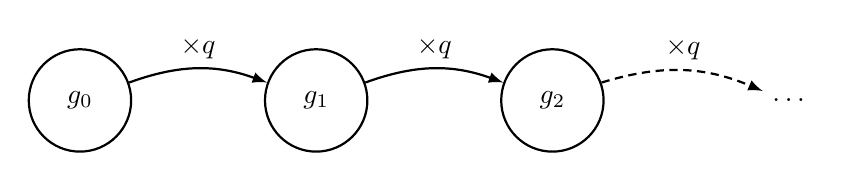
\begin{tikzpicture}[scale=1]
\node[draw,circle,thick, minimum size=13mm] (W0) at (-3,0) {$g_0$};
\node[draw,circle,thick, minimum size=13mm] (W1) at (0,0) {$g_1$};
\node[draw,circle,thick, minimum size=13mm] (W2) at (3,0) {$g_2$};
\node (W5) at (6,0) {$\ldots$};
\draw[->,>=latex,thick] (W0) to[bend left=20] node[midway,above]{$\times q$} (W1);
\draw[->,>=latex,thick] (W1) to[bend left=20] node[midway,above]{$\times q$} (W2);
\draw[->,>=latex,thick,densely dashed] (W2) to[bend left=20] node[midway,above]{$\times q$} (W5);
\end{tikzpicture}
\end{center}
\end{defin}

\begin{rmq}
On passe d'un terme au suivant en multipliant toujours par le même nombre. Le quotient de deux termes successifs vaut toujours $q$: $\frac{g_{n+1}}{g_n}=q$.
\end{rmq}

\begin{ex}
ex
\end{ex}

\subsection{Variations des suites géométriques}

\begin{prop}
\begin{itemize}
\item Si $q > 1$, alors la suite $g$ est croissante.
\item Si $0< q < 1$, alors la suite $g$ est décroissante.
\item Si $q = 1$, alors la suite $g$ est constante.
\end{itemize}
\end{prop}

\begin{ex}
\end{ex}

\begin{deroule}
\item \textbf{Total: 3.5 semaines}
\item Semaine 1
\begin{itemize} 
\item 30m - Cours I partie 1: Définitions et exo
\item 15m - Graphe de $x \mapsto x^2$
\item 1h - Cours: Représentation graphique, sommet, variations, exo
\item 30m - Cours II: Généralités+Exos
\end{itemize}
\item Semaine 2
\begin{itemize}
\item 1h - Suite
\item 1h - II.2 + Exos
\item 45m - III.1.1 + Exos
\item 45m - III.1.2 + Exos
\end{itemize}
\item Semaine 3
\begin{itemize}
\item 30m - Suite
\item 45m: III.1.3 + Exos
\item 1h: III.2 + Exos
\item 1h: III.3 + Exos
\end{itemize}
\end{deroule}

\end{document}
